% Seção 9: Esboço da estrutura mecânica

\section{Esboço da estrutura mecânica}

O esboço da estrutura mecânica é apresentado na Figura~\ref{fig:mecanica}.

\begin{figure}[H]
  \centering
  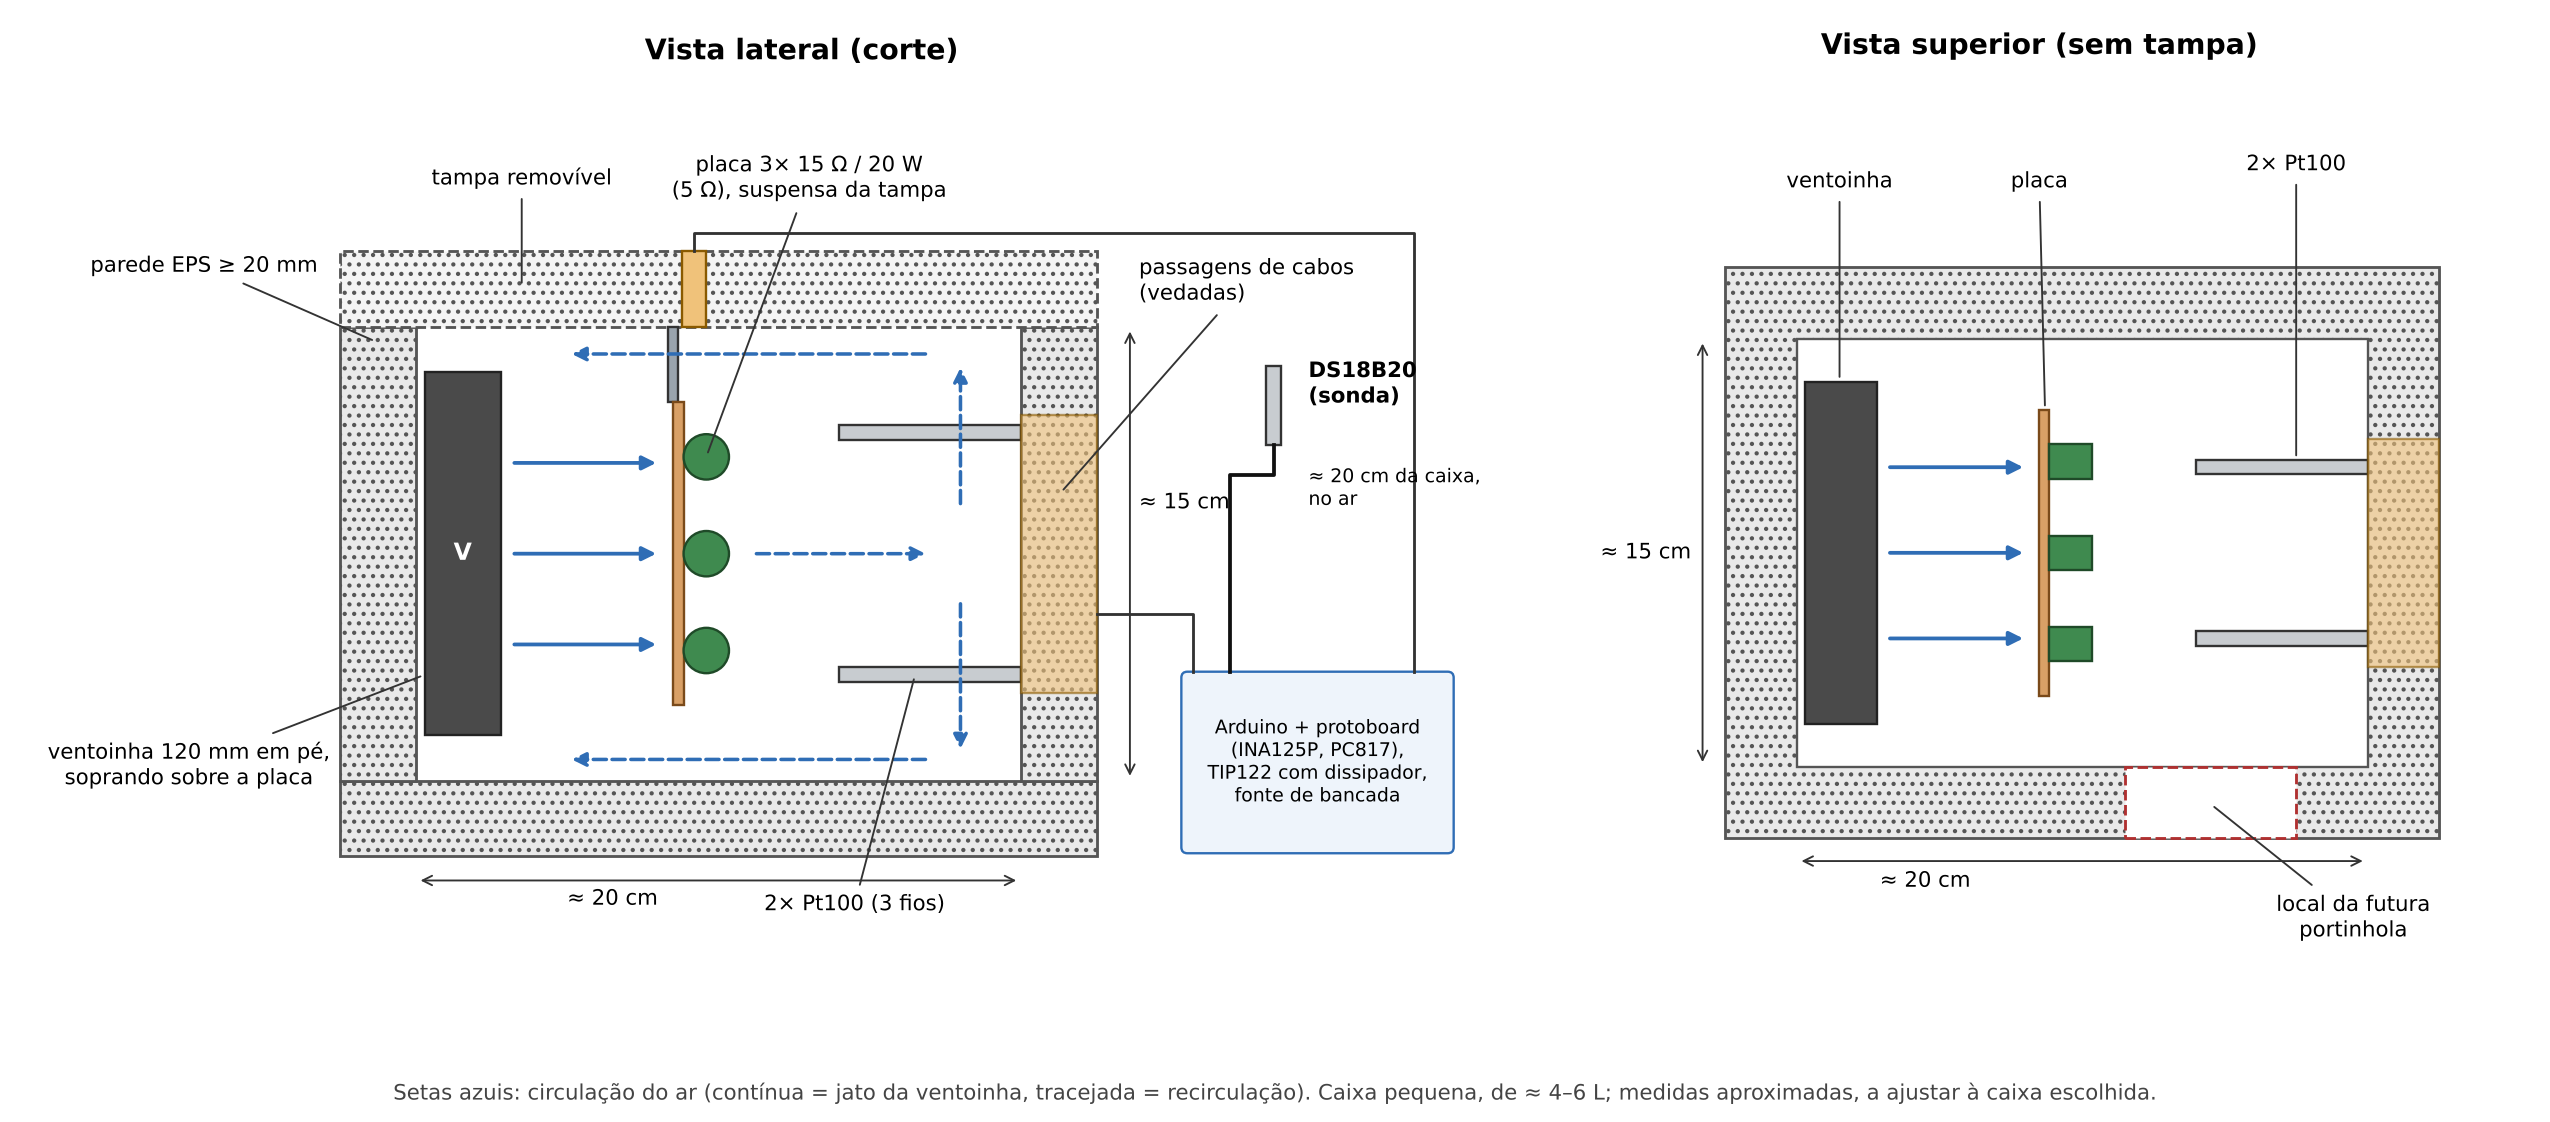
\includegraphics[width=\textwidth]{esboco_mecanico.png}
  \caption{Esboço da estrutura mecânica da câmara térmica: vista lateral em corte e vista superior sem tampa (medidas aproximadas).}
  \label{fig:mecanica}
\end{figure}

\begin{itemize}
  \item \textbf{Câmara:} caixa de EPS pequena, com tampa removível e dimensões internas da ordem de 20\,$\times$\,15\,$\times$\,15\,cm (cerca de 4 a 6\,L), a serem ajustadas à caixa escolhida. As paredes têm pelo menos 20\,mm.
  \item \textbf{Aquecedor:} a placa com os três resistores fica suspensa por um suporte metálico preso à tampa, sem encostar no EPS, com folga de alguns centímetros até as paredes. Os cabos de alimentação saem por um furo na tampa.
  \item \textbf{Ventoinha:} a ventoinha de 120\,mm fica em pé junto a uma parede lateral, soprando o ar diretamente sobre os resistores. O ar aquecido recircula pela tampa, pelo fundo e pelas paredes.
  \item \textbf{Pt100:} os dois sensores entram pela parede oposta, a alguns centímetros da placa, para medir a temperatura do ar da câmara e não a superfície dos resistores.
  \item \textbf{Fora da câmara:} ficam a sonda DS18B20, o Arduino, a protoboard com os circuitos, o TIP122 com dissipador na barra de terminais e a fonte de bancada. As passagens de cabos são vedadas com cola quente.
  \item \textbf{Perturbação:} uma das paredes tem previsto o local de uma futura portinhola, que poderá ser aberta para gerar perturbações nas próximas etapas. A segunda ventoinha disponível poderá soprar ar ambiente por essa abertura.
\end{itemize}
